\newpage

\begin{figure}[H]
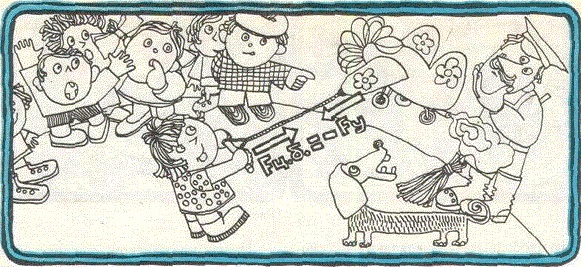
\includegraphics[width = 1\textwidth]{image}
%{\caption*{pic\_7}}
\caption {}
\label{fig:pic_1}
\end{figure}

 \vspace*{5mm} 
\begin{multicols}{2}
\setcounter{page}{34}
% the sum from  i = 1 to N
\sum\limits_{i=0}^N

 
\quad
Здесь уместно заметить, что существует досадная двусмысленность в сложившейся терминологии. Дело в том, что в неподвижной системе от счета силу, с которой движущаяся по окружности материальная точка действует (по третьему закону Ньютона) на тело, удерживающее ее на окружнести (на пружину в нашем примере), называют также центробежной силой. С этой силой никогда не надо путать центробежную силу инерции (это последнее, самое главное слово часто опускают), которая действует на любое тело во вращающейся (неинерциальной) системе отсчета. Эти две силы проявляются в разных системах отсчета и приложены к разным телам (рис.\ref{fig:pic_1}).

\vspace*{3mm}
\setlength\parindent{0pt}
\textbf{Потенциал поля\\ центробежных сил инерции}\\
Подсчитаем работу, которую совершает поле Центробежных сил инерции по перемещению материальной точки массой m. Пусть начальная координата точки (расстояние от оси вращения) равна $r_1$ конечная $r_2$. Центробежная сила инерции равна $m\omega^2$ и направлена от оси вращения.
Если $r_1 - r_2$ мало, то можно записать
$$A=F_{\iy.\ts} \Delta r=m\omega^2\frac{r_1+r_2}{2}\Delta r,$$
заменнв среднюю силу $F_\iy.\ts$ силой в средней точке. Подставив вместо $\Delta r$ значение $r_2 - r_1$, получим
$$A=\frac{m\omega^2r_2^2}{2}-\frac{m\omega^2r_1^2}{2}.$$
\quad
С другой стороны, работа всегда равна изменению потенциальной энергии, взятому $с$ обратным знаком, то есть
$$A=-(\Po_2'-\Po_1').$$
Сравнивая два выражения для работы‚ заметим, что величину
$$\Po'=-\frac{m\omega^2r^2}{2}$$
можно назвать потенциальной энергией материальной точки в поле центробежных сил инерции. а величину $\varphi '=-\frac{\omega^2r^2}{2}$ - соответственно потенциалом этого поля.\\
\quad 
Тогда для вращающейся системы отсчета полная энергия точки при движении равна
$$E'=\frac{mv'^2}{2}-\frac{m\omega^2r^2}{2}$$
и величина ее остается постоянной.\\
\quad
Напомним, однако, что во вращающейся системе отсчета действует еще одна сила инерции (сила Корполиса), зависящая от скорости материальной точки. Поэтому, для того чтобы записать уравнение второго за-
\end{multicols}


\newpage
\vspace*{5mm}
\setcounter{page}{42}

\begin{center}
\begin{tabular}{|l|*{4}{c|}}\hline
\backslashbox{стороны}{случаи}
&\makebox[3em]{I}&\makebox[3em]{II}&\makebox[3em]{III}&\makebox[3em]{IV}\\\hline
AB & 15/4 & 30/13 & 60/13 & 3 \\
BC &  5/4 & 20/13 & 20/13 & 2 \\
CD & 15/4 & 60/13 & 30/13 & 3 \\
DA &  5/4 & 20/13 & 20/13 & 2 \\\hline
\end{tabular}
\end{center}











